\section{Theoretische Grundlagen}
\subsection{Was sind Emotionen?}
Hier soll der Begriff emotionen erklärt werden. Siehe \cite{Sch13}.
\subsection{Welche Möglichkeiten gibt es?}
\subsubsection{Nutzerinteraktionen}
Im Laufe des Alltags verwenden Nutzer ihr Smartphone sehr häufig. Dabei können unteranderem Aspekte wie das Tippverhalte, 
z. Bsp. verwendet der User viele Smileys, Rückschlüsse auf den emotionalen Zustand eines Nutzers ermöglichen.
\subsubsection{Im Smartphone eingebaute Sensoren}
\subsubsection{Zusätzliche Hardware}
Im Rahmen des Projektes wird die Möglichkeit erforscht, mit Hilfe eines Arduinos die Hautleitfähigkeit aufzuzeichnen. 
Diese ist ein großer Faktor bei der Bestimmung von Emotionen und wird unteranderem auch in Lügendetektoren verwendet. 
\begin{figure}[h]
	\centering
	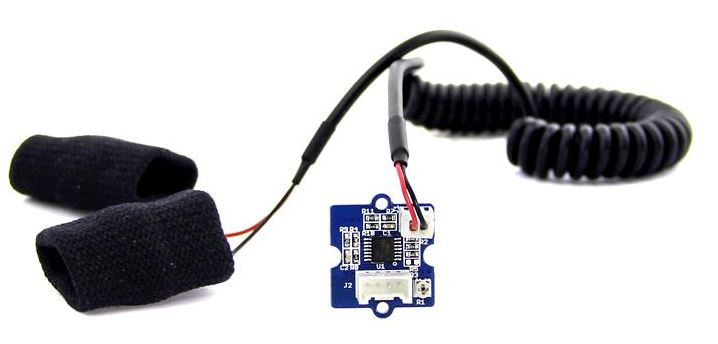
\includegraphics[width=11cm]{Bilder/sensor.jpg}
	\caption{Das ist ein cooler GSR Sensor}
\end{figure}%